\documentclass[spanish]{ieee_upb}

\usepackage{layouts}
\usepackage{caption}
\usepackage{float}

% Información del documento (sin cambios)
\title{APLICATIVO MÓVIL PARA EL AUTOPRÉSTAMO DE LIBROS EN LA BIBLIOTECA BENEDICTO XVI}
\date{\the\year}

\begin{document}
\setlength{\headheight}{15pt}

% Portada (Página 1)
\portada{APLICATIVO MÓVIL PARA EL AUTOPRÉSTAMO DE LIBROS EN LA BIBLIOTECA BENEDICTO XVI}
{ALEXANDRA BERNAL ESCALANTE, NICOLLE FABIANA CADAVID NOGUERA}
{ESCUELA DE INGENERÍAS}
{FACULTAD DE INGENIERÍA DE SISTEMAS E INFORMÁTICA}

% Contraportada (Página 2)
\newpage
\contraportada{APLICATIVO MÓVIL PARA EL AUTOPRÉSTAMO DE LIBROS EN LA BIBLIOTECA BENEDICTO XVI }
{ALEXANDRA BERNAL ESCALANTE, NICOLLE FABIANA CADAVID NOGUERA}
{INGENIERO DE SISTEMAS E INFORMÁTICA}
% MSc NOMBRE
{Mgtr. ELKIN ALFREDO ALBARRACIN NAVAS}
{ESCUELA DE INGENIERÍAS}
{FACULTAD INGENIERÍA DE SISTEMAS E INFORMÁTICA}
% Dedicatoria
\newpage
\section*{DEDICATORIA}
Texto de la dedicatoria...

% Agradecimientos
\clearpage
% Usa el comando specialsection para Agradecimientos
\section*{AGRADECIMIENTOS}
Texto...

% Tabla de contenido
%\pagenumbering{roman} 
\clearpage
\renewcommand\contentsname{\hfill\normalfont\bfseries CONTENIDO\hfill}
\tableofcontents

% Lista de tablas
% Números romanos en las tablas
\renewcommand{\thetable}{\Roman{table}}

% Crear un nuevo contador para el índice
\newcounter{tabindexcounter}

% Personalizar el índice de tablas
\makeatletter
\renewcommand{\numberline}[1]{%
  \stepcounter{tabindexcounter}%
  Tabla~\arabic{tabindexcounter}~%
}
\makeatother

% Formato para el caption de la tabla
%\captionsetup[table]{labelsep=newline, labelfont=bf, name=TABLA}

\newpage
\newcounter{mytablecounter} 
\renewcommand\listtablename{\hfill\normalfont\bfseries LISTA DE TABLAS\hfill}
\listoftables

% Lista de figuras
\newpage
\renewcommand\listfigurename{\hfill\normalfont\bfseries LISTA DE FIGURAS\hfill}
\listoffigures

\clearpage
\renewcommand\lstlistlistingname{\hfill\normalfont\bfseries LISTA DE PSEUDOCÓDIGOS\hfill}
\renewcommand{\lstlistingname}{Pseudocódigo}
\lstlistoflistings

\newpage
\section*{GLOSARIO}
\textbf{CTIC: } Centro de tecnologías de información y comunicaciones.

\vspace{0.1cm}
\textbf{DBSM: } Database Management System (Sistema de Gestión de Base de Datos).

\vspace{0.1cm}
\textbf{IAIN: } Islamic state institute.

\vspace{0.1cm}
\textbf{ISO: } International Organization for Standardization.

\vspace{0.1cm}
\textbf{RFID: } Radio Frequency Identification.

\vspace{0.1cm}
\textbf{SQL: } Structured Query Language. 

\vspace{0.1cm}
\textbf{UMUX: } Usability Metric for User Experience.

\vspace{0.1cm}
\textbf{UNAM: } Universidad Nacional Autónoma de México.

\vspace{0.1cm}
\textbf{UPB: } Universidad Pontificia Bolivariana.

\vspace{0.1cm}
\textbf{UX: } User Experience (Experiencia de usuario).

% Upload resumes in pdf_resumes folder
% THIS MUST BE SIGNED BY DIRECTOR
% visit: https://herramientasbib.bucaramanga.upb.edu.co/resumenesp
% visit: https://herramientasbib.bucaramanga.upb.edu.co/resumening


% Introducción
\newpage
\section{INTRODUCCIÓN}
El proceso de préstamo de libros en la Biblioteca Benedicto XVI de la Universidad Pontificia Bolivariana, seccional Bucaramanga, actualmente se realiza de forma manual por los bibliotecarios, atendiendo a cada uno de los usuarios de la biblioteca. Sin embargo, acorde con la intención de facilitar la adquisición de material bibliográfico para los usuarios y de implementar tecnología como forma de innovar y de mantener a la biblioteca a la vanguardia de la educación, se requiere de herramientas tecnológicas que actualicen los procesos tradicionales.
\vspace{0.3 cm}

Atendiendo a estas razones, el presente proyecto propone el diseño, desarrollo y despliegue de un aplicativo móvil que permita a los usuarios de la biblioteca poder realizar los procesos de autopréstamo de libros, renovación de libros y seguimiento a los préstamos realizados.
\vspace{0.3 cm}

Durante el desarrollo se adoptó el marco de trabajo Scrum con ciclos iterativos de entrega, en los que se realizaban reuniones con la jefatura de biblioteca. En conjunto, como metodología, se adoptaron las metodologías ágiles, dividiendo el proyecto en cinco fases: planificación, diseño, desarrollo, pruebas de software e implementación.
\vspace{0.3 cm}

La implementación del aplicativo móvil para el autopréstamo de libros en la Biblioteca Benedicto XVI permitirá a los usuarios de la biblioteca realizar el autopréstamo de libros mediante el escaneo del código de barras, atendiendo a la misión y visión de la biblioteca por facilitar el material bibliográfico para la formación integral de los usuarios, siendo el eje de toda la actividad académica.
\vspace{0.3 cm}


% Generalidades

% Planteamiento del problema
\newpage
\section{PLANTEAMIENTO DEL PROBLEMA}
Actualmente, los procesos de  transformación digital al interior de las instituciones se apalancan en el buen uso y aprovechamiento de las tecnologías de información como apoyo en los procesos y operaciones existentes, permitiendo una mejora en los mismos y generando procesos innovadores que impactan positivamente en el entorno en el cual las instituciones se desempeñan.  
\vspace{0.3 cm}

En el ámbito bibliotecario, el uso de aplicaciones móviles para ofrecer servicios, se ha convertido en una necesidad y su implementación ha incrementado a partir del 2021, como un efecto de la pandemia, ya que para los usuarios es más cómodo acceder a estos servicios desde su celular, como se menciona en el artículo “Mobile Apps–Based Applications in Libraries and Information Centers: A Systematic Review of the Literature and Future Research Agendas”. \cite{singh2023mobile}
\vspace{0.3 cm}

Teniendo en cuenta lo anterior, al año 2025 la biblioteca Benedicto XVI de la Universidad Pontificia Bolivariana seccional Bucaramanga, no cuenta con algún tipo de herramienta tecnológica de software que los usuarios puedan utilizar para acceder a los servicios de la biblioteca; el único medio tecnológico existente es el servicio web de Alejandría, en el cual los usuarios pueden realizar búsquedas de material. 
\vspace{0.3 cm}
    
El  proceso actual de préstamo de libros se realiza por medio de los bibliotecarios, en donde ellos se encargan manualmente de hacer el registro de cada uno de los libros que se prestan, escaneando el código de barras del texto , teniendo una duración en promedio de 3 a 5 minutos por libro. Lo anterior representa un problema cuando más de cinco estudiantes aguardan en una fila para prestar más de un libro, ya que esta situación supera la capacidad de atención de los bibliotecarios, generando congestión y tiempos de espera prolongados.
\vspace{0.3 cm}

En distintas instituciones de educación superior, con el fin de buscar soluciones tecnológicas que ayuden a optimizar procesos administrativos, se está implementando sistemas de autopréstamo digital, en donde el usuario por medio de una aplicación móvil gestiona por sí mismo el préstamo de libros. Como es el caso de la Universidad Nacional Autónoma de México, que cuenta desde el 2021 con su aplicativo móvil llamado “Bibliotecas UNAM” y la Universidad Carlos III de Madrid siendo uno de los primeros en implementar este tipo de tecnologías que se convirtieron en soluciones para ofrecer un mejor servicio en el préstamo de textos desde el año 2012.
\vspace{0.3 cm}

Por lo anterior, se puede determinar que, teniendo en cuenta las necesidades de la Universidad Pontificia Bolivariana Seccional Bucaramanga, surge la pregunta problema: \textit{¿Cómo mejorar el servicio de préstamo de libros en la Universidad Pontificia Bolivariana Seccional Bucaramanga implementando tecnologías innovadoras de gestión de información?}


% Justificación
\newpage
\section{JUSTIFICACIÓN}

En la actualidad, la innovación e implementación de las tecnologías digitales en los diferentes contextos educativos se ha convertido en un factor clave para la actualización de procesos. Acorde a esto, la Biblioteca Benedicto XVI, en su interés por mantenerse a la vanguardia en el apoyo a la comunidad universitaria de la Universidad Pontificia Bolivariana, seccional Bucaramanga, propone soluciones tecnológicas para modernizarse y brindar mayor accesibilidad a los recursos presentes en ella.
\vspace{0.3 cm}

Dado lo anterior, y considerando el presupuesto limitado para implementar tecnologías más avanzadas como el sistema RFID, se propone el desarrollo de un aplicativo móvil que permita realizar autopréstamos de libros. Esta solución busca modernizar los procesos fundamentales de la biblioteca, alineándose con su estrategia de innovación. El aplicativo busca generar una reducción de tiempos y mejora  en la experiencia de los usuarios finales , facilitándoles el proceso de préstamo y renovación de libros mediante el uso de sus dispositivos móviles.  
\vspace{0.3 cm}

Teniendo en cuenta que actualmente existen mediciones empíricas(estimadas por los bibliotecarios), esta implementación permitirá establecer una línea base para la estimación formal de tiempos del proceso que permita a futuro apoyar la toma de decisiones con respecto  al mismo.
\vspace{0.3 cm}

El desarrollo de esta aplicación representará un avance significativo en la adopción de nuevas tecnologías como medio para mejorar la experiencia de los miembros de la comunidad universitaria. Asimismo, contribuirá a fortalecer el vínculo entre la Biblioteca Benedicto XVI y sus usuarios, incentivando el uso y aprovechamiento del material bibliográfico disponible.
\vspace{0.3 cm}


% Objetivos
\newpage
\section{OBJETIVOS}

\subsection{Objetivo general}

Implementar un aplicativo móvil que permita automatizar el proceso de auto préstamo de libros en la biblioteca Benedicto XVI de la Universidad Pontificia Bolivariana, seccional Bucaramanga.
\subsection{Objetivos específicos}

\begin{itemize}
\item Identificar los requerimientos del sistema mediante la recopilación de información y la evaluación de las necesidades de la biblioteca, para establecer las especificaciones técnicas y funcionales del aplicativo.   
\item Diseñar la arquitectura tecnología del aplicativo móvil a través del uso de diagramas y herramientas de diagramación para representar la arquitectura, implementación, funcionalidad y estructura del sistema.
\item Desarrollar el aplicativo móvil que permita gestionar el proceso de autopréstamo de libros utilizando para ello una arquitectura de tecnológica apoyada en el uso de tecnologías móviles y procesos de lectura de códigos de barras.
\item Implementar el aplicativo móvil en la biblioteca Benedicto XVI para asegurar su correcto funcionamiento dentro del entorno institucional de acuerdo con los requerimientos establecidos y aprobados.

\end{itemize}

% Marco referencial
\newpage
\section{MARCO REFERENCIAL}

\subsection{Antecedentes}
El artículo \textit{Analysis of user satisfaction on self-loan services in Islamic state institute (IAIN) purwokerto library} \cite{antasaria2019analysis} , publicado en el año 2019, evalúa la satisfacción de los estudiantes respecto al servicio de autopréstamo en la biblioteca de IAIN Purwokerto. Por medio de un enfoque cuantitativo, analiza los distintos factores que influyen en la experiencia de usuario, como lo es la facilidad de uso y la accesibilidad del sistema. Una de sus principales conclusiones es que la automatización de los préstamos ha ayudado a mejorar la comodidad de los estudiantes, ayudándoles a acceder al material de manera más fácil. 
\vspace{0.3 cm}

Este artículo menciona la relación existente entre la satisfacción del usuario y la implementación de tecnologías en bibliotecas académicas, en donde el éxito de estas depende de la facilidad que tenga el usuario de interactuar con ellas y que su uso no dependa un conocimiento técnico en tecnologías. 
\vspace{0.3 cm}

Por otro lado, el artículo \textit{Aplicación móvil “Biblioteca UNAM”. Llévala en tu bolsillo }\cite{martinez2021aplicación} describe la implementación de una aplicación móvil que tiene como objetivo brindar acceso a los servicios bibliotecarios de la Universidad Nacional Autónoma de México (UNAM). En donde, los usuarios a través de la plataforma pueden gestionar el préstamo de libros, consultar catálogos y buscar la disponibilidad de libros a través de su dispositivo móvil. 
\vspace{0.3 cm}

El artículo resalta la importancia de la digitalización de las bibliotecas académicas, teniendo en cuenta que, \textit{“proporcionar servicios bibliotecarios por medio de tecnologías de vanguardia a través de dispositivos móviles que ofrecen ventajas en costo, uso y movilidad, que otros no proporcionan”} \cite{martinez2021aplicación}, ayuda a incrementar la satisfacción de los usuarios y optimizar los procesos en la prestación de servicios. 
\vspace{0.3 cm}

El trabajo de investigación: \textit{“Sistema de Gestión y control de préstamos de libros en bibliotecas para teléfonos móviles Android”} de la Universidad Carlos III de Madrid , tiene como objetivo principal implementar un sistema que facilite la gestión de préstamo de libros de una forma más sencilla. En este estudio se resalta la importancia de desarrollar nuevas soluciones tecnológicas que estén alineadas con el auge de la tecnología, ya que “\textit{las aplicaciones móviles permiten ofrecer servicios bibliotecarios personalizados y accesibles en cualquier momento y lugar, optimizando así la relación entre los usuarios y las bibliotecas”} \cite{fombellida2012sistema}. De este modo, fomentar el interés de los estudiantes de utilizar los servicios que ofrece la biblioteca.  
\vspace{0.3 cm}

Por otra parte, la investigación también resalta la importancia de diseñar interfaces atractivas y funcionales para el usuario, ya que es un factor influyente a la hora de determinar si la aplicación suple el proceso que se quiere automatizar y optimizar. 
\vspace{0.3 cm}

El informe Tendencias de innovación en bibliotecas académicas en Latinoamérica y el Caribe, del año 2024, recopila las tendencias y el progreso en la adopción de tecnologías en las bibliotecas académicas de la región, en relación con las principales tendencias internacionales. Este documento analiza la transformación que ha experimentado el sector bibliotecario en los últimos años para mantenerse a la vanguardia mediante la adopción de nuevas estrategias que le permitan responder a los desafíos del entorno. Asimismo, proporciona una visión clara para orientar a los líderes bibliotecarios en su adaptación a los cambios en el ámbito educativo y tecnológico.
\vspace{0.3 cm}

El informe ofrece una visión general sobre cómo la integración de las tecnologías representa un avance y una mejora en los servicios de las bibliotecas académicas:``En el ámbito tecnológico, se evidencia que los nuevos desarrollos e innovaciones facilitan a las bibliotecas universitarias la adopción de estrategias basadas en tecnología para mejorar sus servicios y adaptarse a los cambios en el entorno.''\cite{unal_87281}
\vspace{0.3 cm}

Acorde a las tendencias de innovación e integración de estrategias basadas en tecnologías, el trabajo de grado “Desarrollo y personalización de contenidos digitales para la aplicación UPB Móvil a partir de las necesidades comunicacionales encontradas en cada seccional a nivel nacional”, realizado por Yorley Arelys Ruiz Manco y Mitchelle Ivonne Mora Páez, demuestra el interés de la Universidad Pontificia Bolivariana en la adopción de soluciones digitales que resuelvan y optimicen la comunicación institucional, facilitando a los estudiantes el acceso a información relevante y mejorando la eficiencia de los procesos académicos y administrativos a través del uso de herramientas tecnológicas.
\vspace{0.3 cm}

Proyectos como la UPB Móvil \cite{ruiz2017desarrollo} destacan la necesidad de adoptar soluciones tecnológicas con el fin de mejorar la experiencia de los estudiantes y de continuar con el desarrollo e integración de aplicaciones propias de la universidad.
\vspace{0.3 cm}

Finalmente, el trabajo “Desarrollo de un prototipo de aplicativo móvil para bibliotecas: BibliotecApp”, perteneciente a la Especialización en Proyectos Informáticos de la Universidad Distrital Francisco José de Caldas, realizado en el año 2021 por Cristian Camilo Ortega Ardila, ofrece una visión de cómo distintas universidades a nivel nacional están integrando herramientas tecnológicas en sus bibliotecas. Esto responde a la necesidad de adaptación del sector, ya que “la biblioteca universitaria está obligada a reinventarse para acercarse a sus usuarios, facilitando los trámites y garantizando un acceso instantáneo a información pertinente y de calidad”. \cite{ortegadesarrollo}

\subsection{Marco teórico}

\subsubsection{Sistemas de préstamo en bibliotecas}
Las primeras etapas en los sistemas de préstamo en las bibliotecas se realizaban por medio de métodos manuales que se basaban en el uso de fichas de papel, en donde cada libro tenía uno y allí registraban el nombre de la persona, la fecha de los préstamos y la de devolución, estos métodos según Rubin tenían como resultado procesos lentos y no representaba una buena experiencia para el usuario.\cite{rubin2020foundations}
\vspace{0.3 cm}
   
Con la aparición de las computadoras en la década de 1970 empezó el proceso de automatización en las bibliotecas.  Los Sistemas de Gestión de Biblioteca o los ILS se utilizan para automatizar todas las operaciones de las bibliotecas, estos sistemas son organizados en distintos módulos, en donde cada uno de ellos se encargan de tareas específicas, pero comparten una misma base de datos \cite{picco2011manual}. La implementación de estos sistemas permite al usuario al acceso autónomo y directo a la información. 

\subsubsection{Ventajas de los sistemas de Gestión de Biblioteca}

Una de las principales ventajas de los sistemas automatizados es que ayudan a mejorar la eficiencia operativa, en el ámbito de reducir el tiempo a la hora de realizar prestamos, devoluciones y búsquedas. Sadeh en su estudio \textit{Time for a change: new approaches for a new generation of library users} descubrió que la automatización puede reducir el tiempo de búsqueda a un 50\% \cite{sadeh2007time}.
\vspace{0.3 cm}

En el artículo \textit{"Revolutionizing Libraries: A Review of Advanced Library Management Systems"} se destaca que una de las principales ventajas de estos sistemas es que permite realizar los procesos internos de manera más rápida y precisa \cite{Singh2024}. Además, contribuye a disminuir la carga de trabajo del personal bibliotecario, lo que optimiza la prestación de servicios y mejora la experiencia de los usuarios, ya que los servicios se vuelven más accesibles y pueden ser gestionados de manera autónoma. 

\subsubsection{Tecnologías aplicadas en bibliotecas para el préstamo de libros}
Los sistemas de autopréstamo están diseñados para mejorar el proceso de préstamo de libros en bibliotecas mediante la integración de herramientas tecnológicas. Esto agrega valor a la experiencia de los usuarios y permite que las bibliotecas se mantengan a la vanguardia del avance tecnológico. La implementación de estas soluciones tecnológicas fomenta el interés de los usuarios, gracias a los beneficios que ofrecen los sistemas de autopréstamo, como la rapidez, facilidad de uso, autonomía, privacidad y seguridad.\cite{rodriguez2015automatizacion}

\subsubsection{Tecnologías utilizadas en sistemas de autopréstamo}
La implementación de sistemas de autopréstamo implica la incorporación de tecnologías que optimizan el servicio bibliotecario. Una de estas herramientas es el escaneo de códigos de barras, el cual, según Cabral (2019), ha transformado la gestión de recursos en bibliotecas mediante la identificación automática con códigos de barras, códigos QR y tecnología RFID. Esto ha permitido una mejor trazabilidad y control de los materiales bibliográficos, agilizando los procesos de préstamo y devolución. \cite{cabral2017identificacion}
\vspace{0.3 cm}

Otra tecnología clave en la modernización de los servicios bibliotecarios son las aplicaciones móviles, debido a su accesibilidad y facilidad de uso. Su creciente adopción en bibliotecas responde a la necesidad de facilitar el acceso a los servicios bibliotecarios para los usuarios. De acuerdo con Quiroz (2023), estas aplicaciones no solo optimizan la gestión de préstamos, sino que también fomentan una mayor interacción entre la comunidad académica y los recursos bibliográficos disponibles, mejorando la experiencia del usuario y la eficiencia en la administración de los servicios bibliotecarios. \cite{alonso2017aplicaciones}

\subsubsection{Importancia del desarrollo de apps en la gestión bibliotecaria}
En el panorama actual, las bibliotecas académicas enfrentan una transformación digital para mantener su relevancia en la educación superior. Las tendencias indican que están integrando tecnologías emergentes para optimizar la experiencia del usuario, adoptando soluciones como estanterías inteligentes, sistemas de autopréstamo y transmisión de datos para mejorar sus servicios y adaptarse a los avances tecnológicos. \cite{unal_87281}
\vspace{0.3 cm}

Además, las bibliotecas deben responder a las cambiantes expectativas de los usuarios, quienes buscan servicios alineados con las posibilidades que ofrece la tecnología. En este contexto, y en concordancia con la transformación digital, las bibliotecas deben ampliar su oferta incorporando herramientas como videojuegos, música, libros autopublicados y, especialmente, aplicaciones móviles que faciliten el acceso a sus recursos y mejoren la interacción con los usuarios.\cite{gomez2015biblioteca}

\subsection{Marco conceptual}
Teniendo en cuenta los aspectos mencionados en el documento y que hacen parte del proyecto, se derivan algunos conceptos prioritarios a nivel metodológico y de arquitectura tecnológica, los cuales principalmente se asocian a la lógica de negocio del proceso de préstamo de libros y las tecnologías involucradas para lograr una implementación exitosa. Dichos conceptos son:


\subsubsection{Lógica de Negocio: }El presente proyecto tiene como objetivo automatizar el proceso de préstamo de libros mediante un aplicativo móvil, con el fin de mejorar la atención a los usuarios y facilitar el acceso al material bibliográfico disponible en la \textbf{Biblioteca Benedicto XVI}. Esta biblioteca, perteneciente a la Universidad Pontificia Bolivariana, seccional Bucaramanga, cuenta con una colección de aproximadamente 59.000 volúmenes clasificados en colección general, referencia, reserva y trabajos de grado.\vspace{0.3 cm}

Actualmente, el servicio de préstamo permite a estudiantes, docentes y personal administrativo tomar prestados hasta diez libros por un período de un mes. Este plazo puede renovarse a través del portal web institucional, en el apartado de renovaciones. No obstante, este proceso no se encuentra alineado con las tendencias tecnológicas adoptadas por bibliotecas a nivel global, que buscan mantenerse a la vanguardia y continuar desempeñando un papel relevante en la formación profesional \cite{rodriguez2015automatizacion}.\vspace{0.3 cm}

Por esta razón, la integración de soluciones tecnológicas como el sistema de \textbf{autopréstamo de libros}, representa un avance significativo en la modernización de los servicios bibliotecarios. Este sistema automatizado permite a los usuarios realizar el préstamo de libros de manera autónoma, sin la intervención del personal bibliotecario, lo que optimiza el tiempo y los recursos institucionales. A través de su implementación mediante una aplicación móvil, el usuario puede escanear el código de barras del libro deseado, y dicha información queda registrada automáticamente en el sistema, actualizando así el proceso de préstamo.\vspace{0.3 cm}

De esta forma, la Biblioteca Benedicto XVI reafirma su compromiso con la transformación digital, consciente de la necesidad de adaptarse a las nuevas tecnologías para responder a las demandas actuales de la comunidad académica.\vspace{0.3 cm}

El sistema de autopréstamo se basa en la lógica de negocio establecida en el \textbf{software Alejandría}, plataforma mediante la cual la biblioteca se encuentra sistematizada y automatizada. Este software permite gestionar de manera integral todos los procesos internos, tales como: préstamo, devolución y renovación de libros, así como el control de inventario y la búsqueda bibliográfica.\vspace{0.3 cm}

Para una mejor comprensión de la lógica que sustenta este proyecto, a continuación se presenta el diagrama de flujo correspondiente al proceso de préstamo de libros:\vspace{0.3 cm}

\begin{figure}[H]
    \centering
    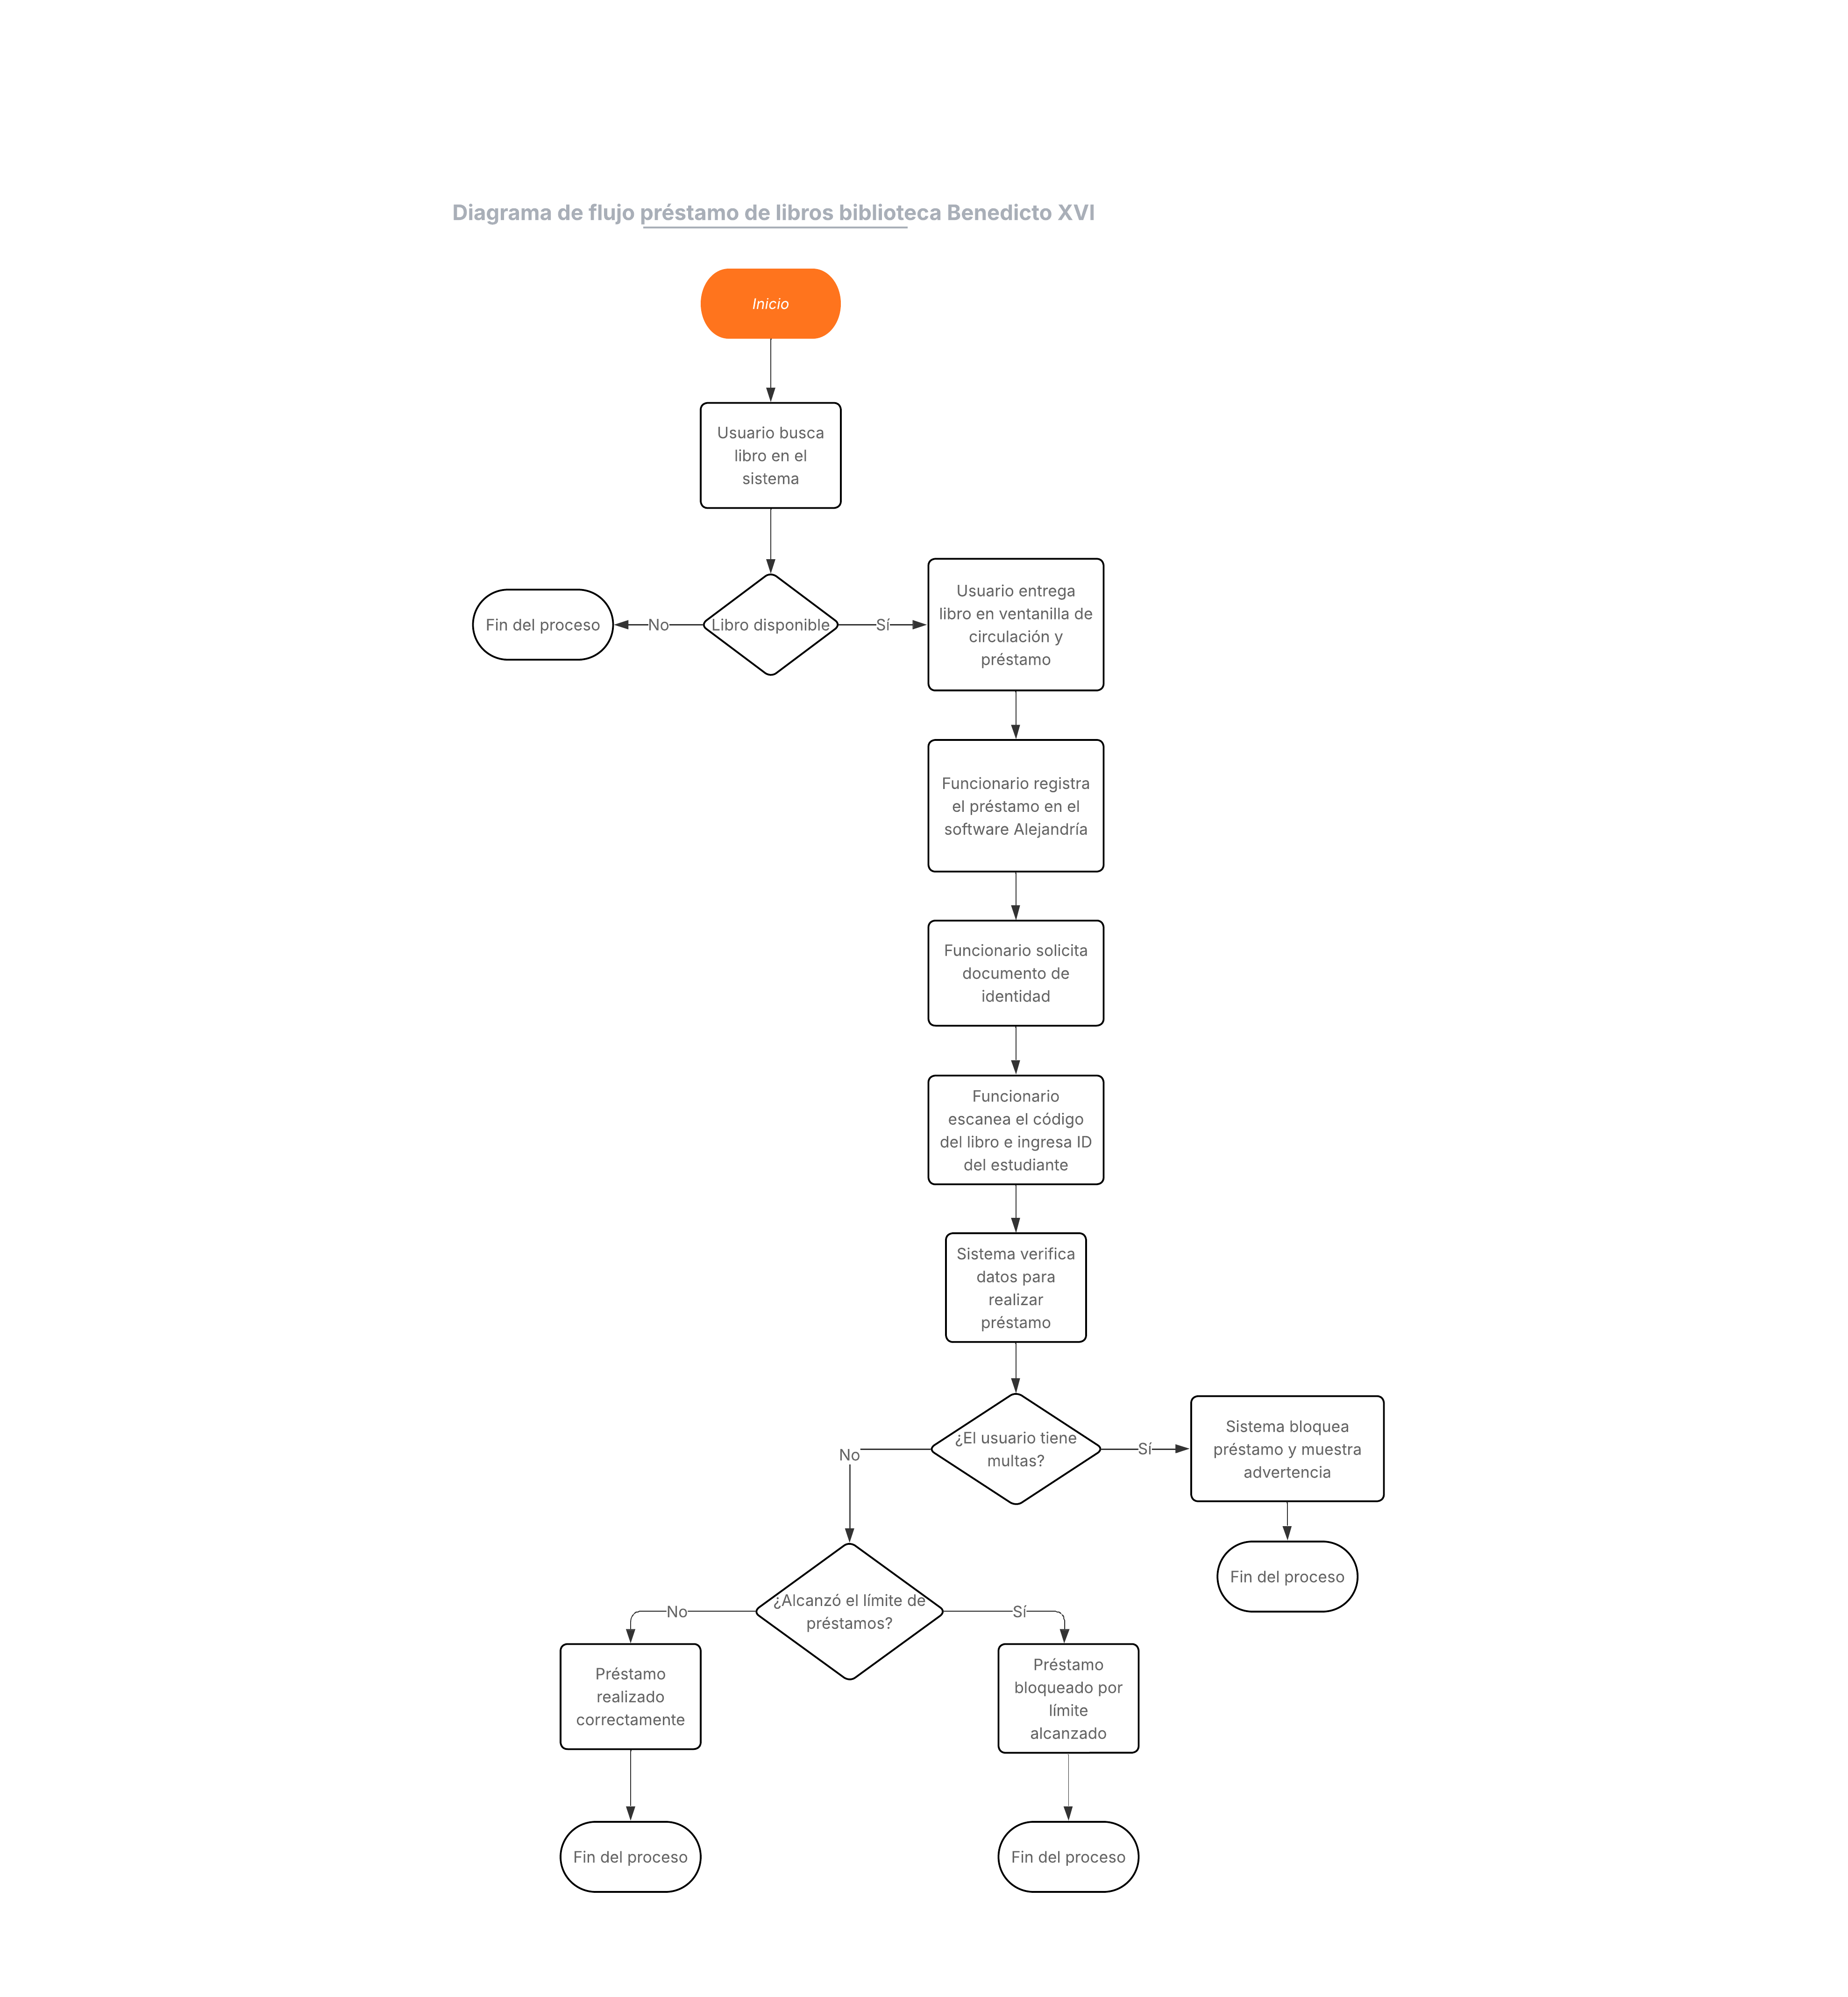
\includegraphics[width=0.9\linewidth]{img/DFpasosPrestamo.png}
    \caption[Préstamo de libros biblioteca Benedicto XVI]{Diagrama de flujo del proceso actual de préstamo de libros}
    \label{fig:presupuesto}
\end{figure}

En la Figura 1 se ilustra el flujo de trabajo actual y la lógica de negocio que se sigue en el proceso de préstamo de material bibliográfico. Inicialmente, el usuario consulta en el sistema la disponibilidad del libro y lo ubica dentro de la colección de la Biblioteca Benedicto XVI. Luego, se dirige a la ventanilla de circulación y préstamo, donde entrega el libro al funcionario de la biblioteca.\vspace{0.3 cm}

El funcionario solicita un documento de identidad para verificar al usuario e ingresa los datos requeridos en el sistema, escanea el código de barras del libro y digita el ID del usuario. Una vez verificada la información, el sistema valida si el usuario cumple con los requisitos para realizar el préstamo. Si el usuario tiene multas activas o ha alcanzado el límite permitido de libros prestados, el sistema no autoriza la operación. En caso contrario, el préstamo se realiza exitosamente y queda registrado en el sistema.\vspace{0.3 cm}

Ahora, con base en esta lógica de negocio, el sistema de autopréstamo actualiza el proceso convencional y elimina la intervención de los funcionarios para efectuar los préstamos. Como se puede observar en la Figura 2, una vez integrado el aplicativo móvil de autopréstamo, el proceso se simplifica.\vspace{0.3 cm}

\begin{figure}[H]
    \centering
    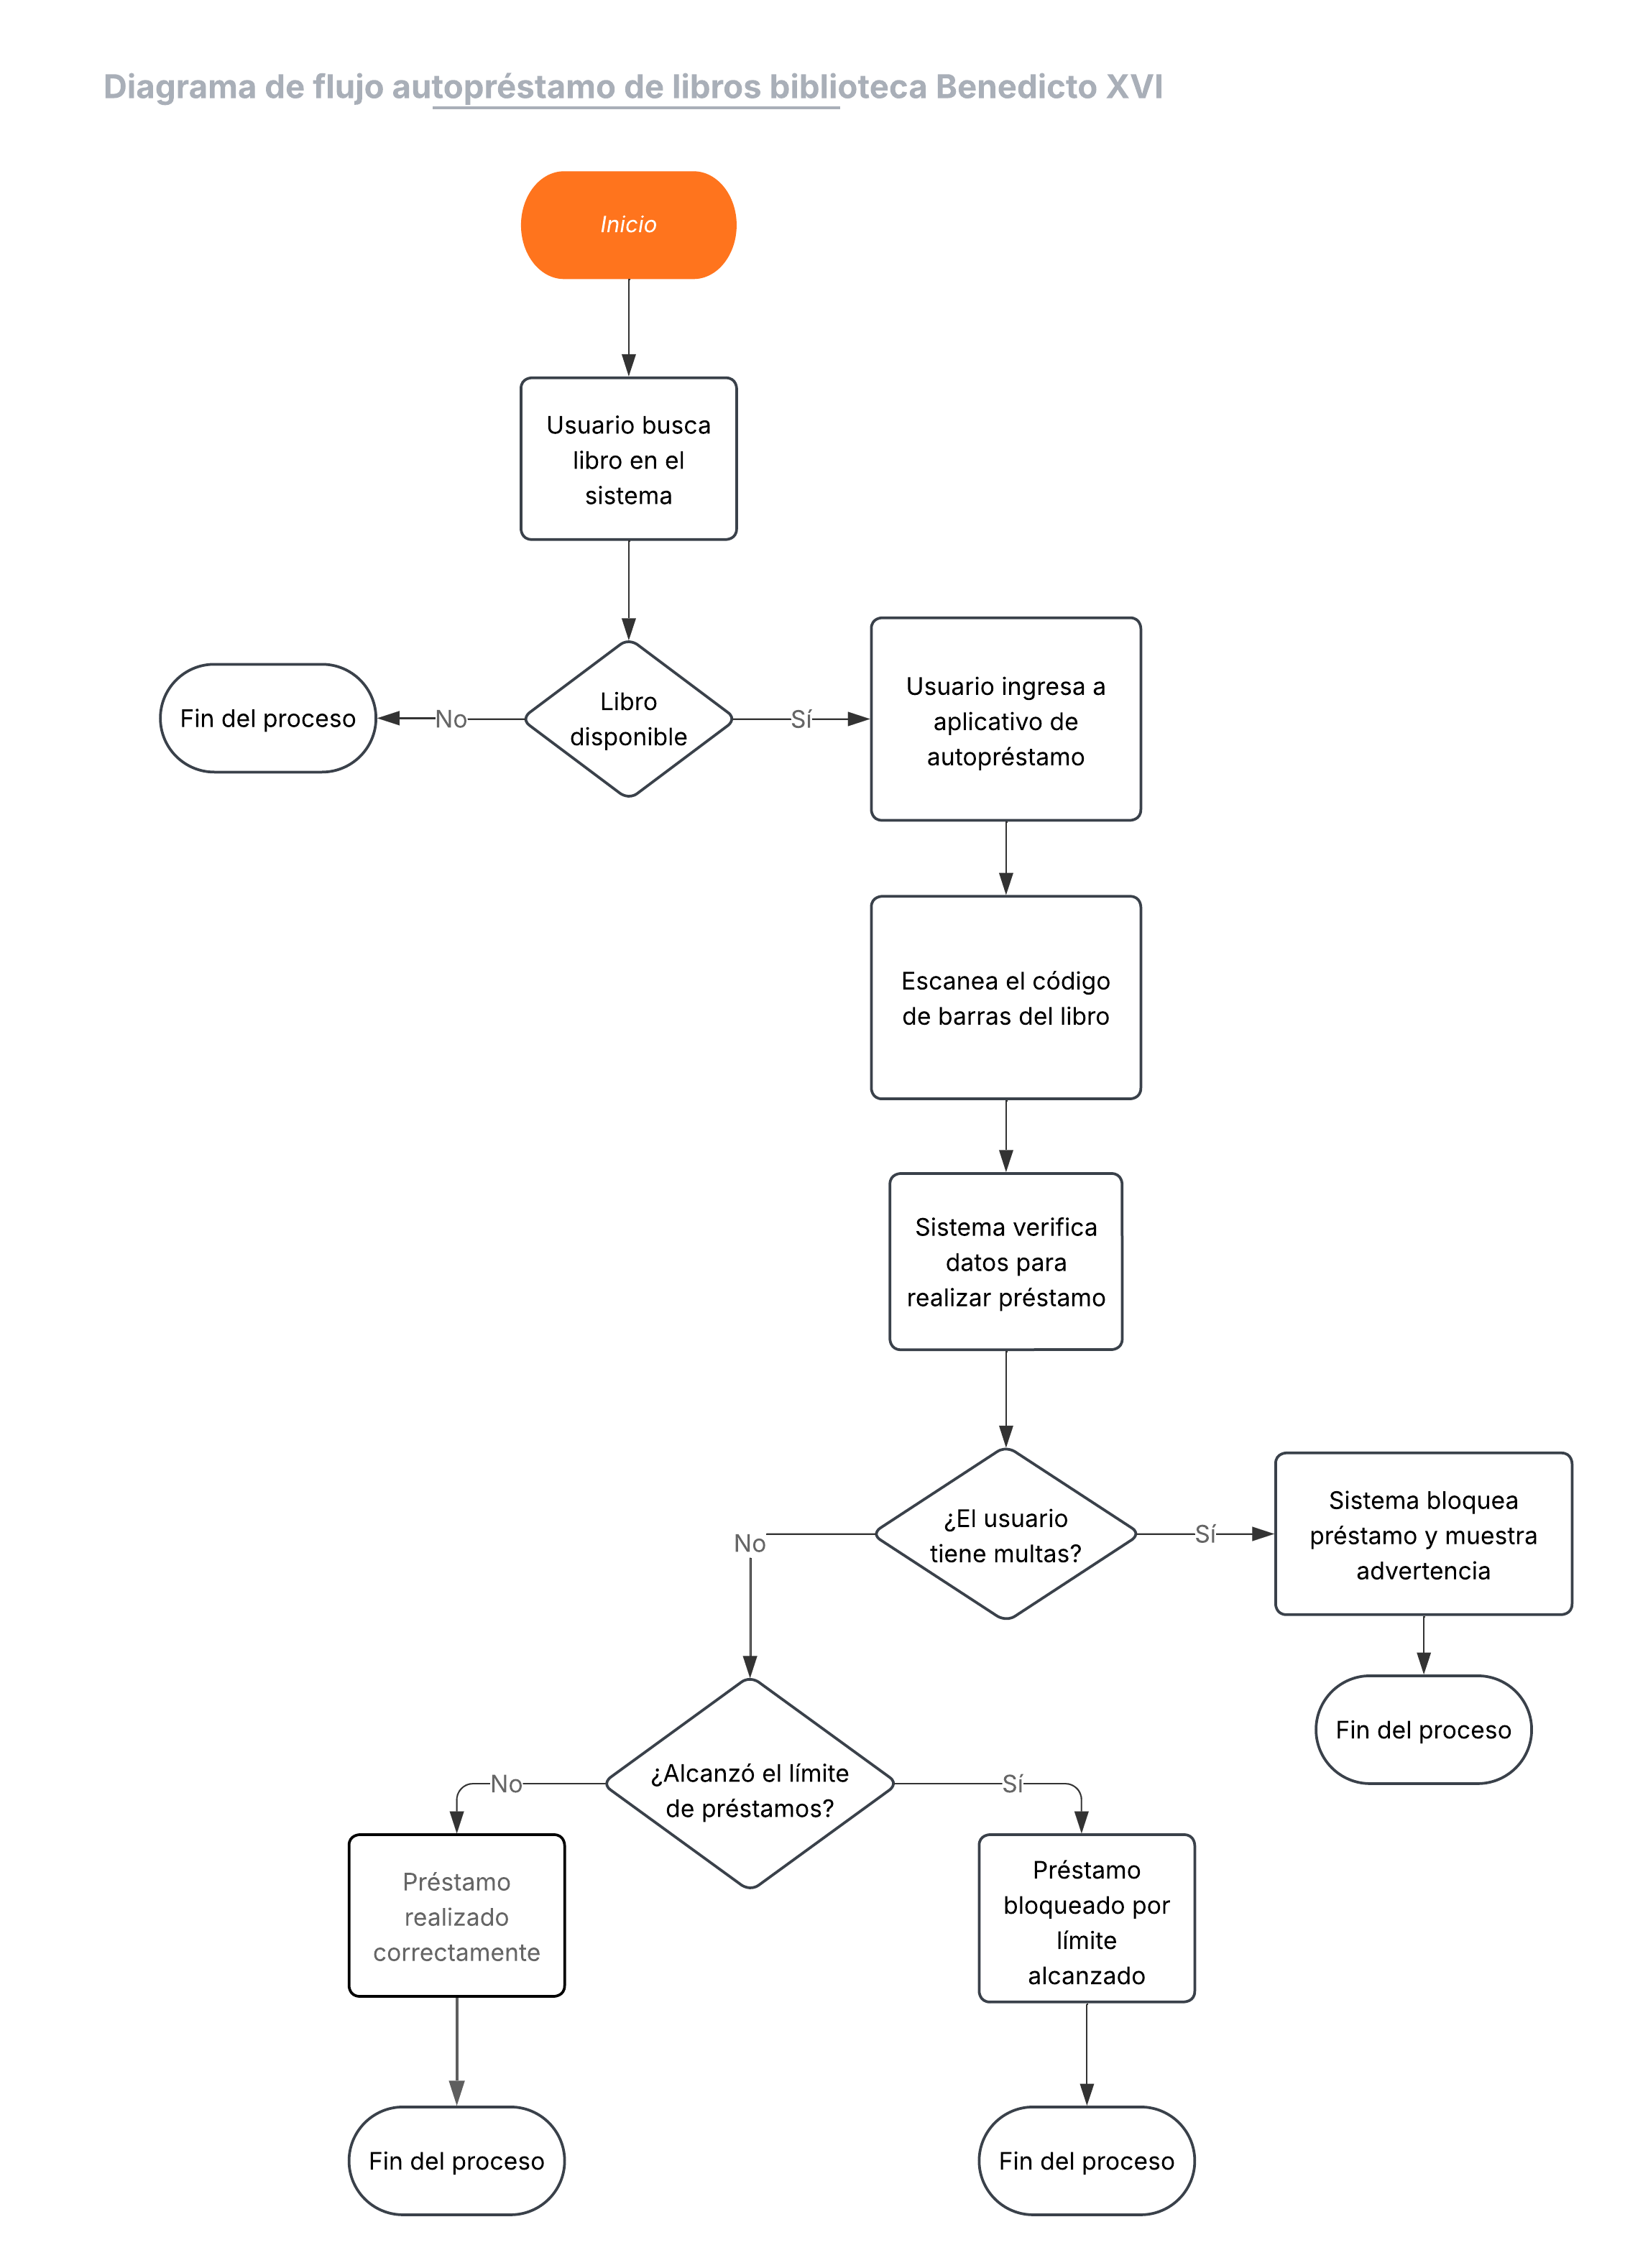
\includegraphics[width=0.7\linewidth]{img/DFpasosAutoPrestamo.png}
    \caption[Préstamo de libros biblioteca Benedicto XVI]{Diagrama de flujo del proceso de autopréstamo}
    \label{fig:FlujoAutoprestamo}
\end{figure}

El proceso actualizado consiste en que el usuario, primero, verifica la disponibilidad del libro, para luego acceder al aplicativo móvil destinado para este fin e iniciar sesión con sus credenciales. A continuación, escanea el código de barras del respectivo libro, tras lo cual el sistema verificará que no se exceda el límite de préstamos permitidos por usuario y que no existan multas activas. Si no hay restricciones, el autopréstamo se efectúa de manera automática.


\subsubsection{Tecnologías Involucradas:} El desarrollo del aplicativo móvil para el autopréstamo de libros en la Biblioteca Benedicto XVI se basa en la integración de diversas tecnologías, tanto de desarrollo como de gestión, que permiten un flujo de trabajo controlado y orientado a obtener un resultado óptimo según la especificación de requerimientos establecida. Por esta razón, es necesario detallar dichas tecnologías para una mejor comprensión del proceso.\vspace{0.3 cm}

El proyecto consiste en el desarrollo de un software diseñado para ejecutarse en dispositivos móviles como teléfonos inteligentes y tabletas, conocido como \textbf{aplicación móvil}. En el marco del proyecto, el servicio de autopréstamo de libros de la Biblioteca Benedicto XVI se presentará a los usuarios por medio de dicho aplicativo. Este software aprovecha funcionalidades como el GPS, la cámara y otros sensores integrados en los dispositivos \cite{IBM_mobile_app_development}, elementos comúnmente utilizados en el desarrollo de aplicaciones destinadas a cubrir diversas necesidades. Estas aplicaciones, por lo general, se distribuyen a través de plataformas como Google Play Store, App Store o Microsoft Store, facilitando el acceso por parte de los usuarios.\vspace{0.3 cm}

La elección de esta tecnología como base del desarrollo del proyecto responde a la necesidad de ofrecer a los usuarios una forma ágil y accesible de interactuar con los servicios de la biblioteca. Dado que los dispositivos móviles representan actualmente uno de los principales medios de conexión a la red, y considerando el interés de la Biblioteca Benedicto XVI por implementar herramientas tecnológicas que fomenten una mayor participación en los procesos de formación académica, el aplicativo móvil de autopréstamo se convierte en una solución adecuada al contexto y objetivos del proyecto.\vspace{0.3 cm}

Específicamente, el aplicativo móvil para el autopréstamo de libros hará uso de la cámara del dispositivo para escanear el \textbf{código de barras} correspondiente a cada libro. Este código es un sistema de representación visual que almacena datos mediante patrones de líneas verticales \cite{economipedia_codigo_de_barras}. En la Biblioteca Benedicto XVI, cada libro cuenta con un código de barras que corresponde a un número de inventario de seis dígitos, el cual lo identifica de forma única en el sistema bibliotecario. Para leer estos códigos, se requiere un dispositivo con capacidad de escaneo; en el marco del proyecto, esta función será asumida por los dispositivos móviles del usuario. De esta manera, cuando el usuario desee tomar prestado un libro, escanea su código y el sistema registra el préstamo.\vspace{0.3 cm}

Adicionalmente, el aplicativo móvil permitirá al usuario visualizar una lista de sus préstamos activos, brindando acceso a información detallada como la fecha de inicio y la fecha de finalización de cada préstamo. Además, se incluirá una opción de redirección al portal web de renovaciones de la Biblioteca Benedicto XVI, con el fin de centralizar los procesos digitales de la biblioteca. Cabe aclarar que las renovaciones no se gestionarán directamente desde el aplicativo móvil, sino que continuarán realizándose a través del portal Alejandría.\vspace{0.3 cm}

No obstante, el aplicativo sí gestionará notificaciones push para recordar al usuario la proximidad del vencimiento del préstamo. Estas notificaciones serán enviadas tres días antes y un día antes de la fecha límite.\vspace{0.3 cm}

El aplicativo móvil será desarrollado para dispositivos Android que cuenten con servicios de Google, específicamente en las versiones 13 y 14 del sistema operativo. Además, se implementará un aplicativo de escritorio cuyo objetivo será verificar los autopréstamos realizados por los usuarios. Esta medida de seguridad ha sido adoptada por los administrativos de la Biblioteca Benedicto XVI con el fin de garantizar una mejor trazabilidad de los préstamos y evitar la pérdida de material bibliográfico.\vspace{0.3 cm}

El aplicativo de escritorio, que será manejado por el funcionario encargado, contará con la función de escanear el código de barras de los libros mediante lectores de radiofrecuencia. Si el libro fue auto prestado correctamente, el sistema mostrará un mensaje confirmando esta acción; en caso contrario, se emitirá una advertencia. Esta función se integra en la lógica de negocio del proyecto como una etapa posterior al autopréstamo, en la cual se espera que el usuario pase por la ventanilla con el libro para que el funcionario verifique la validez del préstamo.\vspace{0.3 cm}

Durante el desarrollo del proyecto se implementará el \textbf{marco de trabajo Scrum} como enfoque metodológico, debido a que permite una planificación adaptable mediante herramientas como el product backlog, la priorización de tareas y la evaluación continua. Este marco estructura el desarrollo en ciclos iterativos y flexibles denominados sprints, lo que facilita la adaptación a los cambios y la mejora continua del producto\cite{schwaber2020guia}. Su implementación permite aplicar principios de las metodologías ágiles en el ámbito del desarrollo de software, promoviendo una gestión colaborativa, adaptable y orientada a resultados.\vspace{0.3 cm}

La aplicación de esta metodología ágil por medio del marco de trabajo scrum se organizará en cinco fases, que abarcan desde la planificación y definición de objetivos hasta la implementación final del sistema en el entorno de producción de la biblioteca. Cada fase contempla tareas específicas, asignadas mediante herramientas de gestión como Jira, GitHub y Excel, utilizadas para el control de versiones, la documentación del proceso y el seguimiento del avance.\vspace{0.3 cm}

Este enfoque ágil permitirá una mayor adaptabilidad frente a la retroalimentación continúa proporcionada por el cliente, y asegurará la entrega de funcionalidades al final de cada sprint, lo cual contribuye al cumplimiento de los objetivos establecidos y a la mejora progresiva del sistema.\vspace{0.3 cm}

El aplicativo móvil de autopréstamo operará bajo una \textbf{arquitectura web} basada en el modelo cliente-servidor, lo que permitirá establecer una comunicación entre los dispositivos móviles de los usuarios (clientes) y el servidor central de la biblioteca. En este modelo, el cliente realiza peticiones específicas y el servidor responde procesando dichas solicitudes, gestionando los datos y retornando la información correspondiente \cite{guillen2019arquitectura}. \vspace{0.3 cm}

El servidor, en este caso, alojará la lógica de negocio del sistema bibliotecario, siendo responsable de operaciones como la validación de préstamos, el registro de transacciones y la verificación de la disponibilidad de libros. Estas operaciones se realizarán mediante una API REST, la cual facilitará el intercambio de información estructurada en formatos como JSON, permitiendo una integración eficiente y estandarizada entre el cliente móvil y el servidor.\vspace{0.3 cm}

La adopción de esta arquitectura web responde a la necesidad de contar con un sistema centralizado, modular y escalable, que pueda adaptarse a futuras funcionalidades y soportar un crecimiento progresivo del número de usuarios. Asimismo, garantiza una mayor flexibilidad para implementar nuevas características sin comprometer la estructura existente del sistema, facilitando el mantenimiento y evolución del servicio a largo plazo \cite{guillen2019arquitectura}.\vspace{0.3 cm}

Finalmente, se hará uso de \textbf{pruebas de software} para evaluar el funcionamiento del aplicativo móvil de autopréstamo. Estas pruebas tienen como objetivo verificar que el sistema cumpla con los requerimientos definidos por el usuario, así como identificar fallos que puedan comprometer su funcionamiento, fiabilidad o usabilidad. Para ello, se aplicarán diferentes tipos de pruebas como las pruebas unitarias, que validan el correcto funcionamiento de componentes individuales; pruebas funcionales, que evalúan el comportamiento del sistema frente a entradas específicas; y pruebas de integración, orientadas a comprobar la interacción entre los distintos módulos del sistema, en especial entre el cliente móvil y el servidor a través de la API REST \cite{kaner1999testing}.\vspace{0.3 cm}

De esta forma, el producto final entregado será coherente con los requerimientos del sistema establecidos en la etapa inicial del proyecto. Además, se implementará el instrumento \textbf{Usability Metric for User Experience (UMUX)} como métrica de evaluación para medir la usabilidad percibida del sistema por parte de los usuarios, permitiendo valorar la experiencia de uso y el nivel de satisfacción frente a la implementación del aplicativo.\vspace{0.3 cm}

UMUX se basa en la definición de usabilidad propuesta por la norma ISO 9241-11, la cual contempla tres componentes fundamentales: efectividad, eficiencia y satisfacción \cite{umux}. Para su aplicación, esta herramienta utiliza cuatro ítems \textit{(ver tabla \ref{tabla:UMUX})}, que el usuario califica mediante una escala de Likert de 7 puntos, indicando su grado de acuerdo o desacuerdo con cada afirmación.

\stepcounter{mytablecounter} % Incrementa el contador personalizado
\addcontentsline{lot}{table}{\protect\numberline{\themytablecounter} UMUX}

\begin{table}[htpb]
    \centering
    \caption[Nombre en la lista de tablas]{\bfseries Componentes de Usabilidad en UMUX }
    \label{tabla:UMUX}
   
    \begin{tabular}{|c|p{11cm}|} \hline 
         \textbf{Componente de Usabilidad}&  \textbf{Ítem candidato de UMUX}\\ \hline 
         Efectividad  & Este sistema cumple con mis requerimientos \\ \hline 
         Satisfacción &Usar este sistema resulta ser una experiencia frustrante \\ \hline 
         General      & Este sistema es fácil de usar \\ \hline
         Eficiencia   & Tengo que dedicar demasiado tiempo en corregir errores con este sistema \\ \hline
    \end{tabular}    
\end{table}



\subsection{Marco Tecnológico}
\subsubsection{Diseño y desarrollo de aplicaciones para Android: }
Las aplicaciones móviles se han consolidado en los últimos años como la herramienta tecnológica predilecta por los usuarios debido a la facilidad de su uso y a la gran variedad que hay en el mercado. Acorde a esta relevancia, Android se ha afianzado como el sistema operativo con mayor crecimiento a nivel global, gracias a su enfoque que fomenta la satisfacción del usuario y el desarrollo de aplicaciones en diversos sectores tales como la gestión bibliotecaria. \cite{Statista2025} \cite{polanco2011android}

\subsubsection{Tecnologías utilizadas en el desarrollo de la aplicación: }
Para el desarrollo del aplicativo móvil de autopréstamo se han seleccionado tecnologías modernas y eficientes que faciliten el desarrollo y garanticen una experiencia fluida para los usuarios de la aplicación y para la gestión de los recursos bibliotecarios. Estas tecnologías incluyen Flutter y Dart para el desarrollo móvil, Node.js y Express para el backend, y GitHub para el control de versiones y la colaboración en el desarrollo.
\vspace{0.3 cm}

\paragraph{\textbf{Flutter y Dart}}
Flutter es un framework multiplataforma diseñado por Google para el desarrollo de aplicaciones móviles de alto rendimiento. Gracias a su motor de renderizado, es posible crear interfaces de usuario atractivas, flexibles y responsivas con facilidad. \cite{tashildar2020application} \cite{Kinari2024}
\vspace{0.3 cm}

Además, Flutter, al ser una tecnología multiplataforma, permite que una misma base de código se adapte a diferentes sistemas operativos, gracias al uso de Dart como lenguaje de programación. Dart ofrece rapidez en la ejecución y facilita el manejo de interfaces reactivas. Es un lenguaje moderno que implementa características del estándar JavaScript (ES7) y adopta una sintaxis similar a la de Java.\cite{tashildar2020application}
\vspace{0.3 cm}

\paragraph{\textbf{Node.js y Express}}
Para el desarrollo del backend de la aplicación se ha optado por Node.js, un entorno de ejecución de JavaScript basado en un modelo asíncrono y orientado a eventos, diseñado para construir aplicaciones de red altamente escalables. \cite{shah2017node} \cite{haro2019desarrollo}
\vspace{0.3 cm}

Entre sus principales ventajas destacan su capacidad para manejar múltiples solicitudes simultáneamente mientras actúa como cliente hacia servicios externos, así como la eliminación de la necesidad de alternar entre diferentes lenguajes de programación en el desarrollo frontend y backend, ya que todo el código se escribe en JavaScript. \cite{shah2017node} \cite{haro2019desarrollo}
\vspace{0.3 cm}

Además, se utilizará el framework web Express.js, el cual está basado en el núcleo de Node.js y ofrece una estructura ligera con una amplia flexibilidad, permitiendo una gran personalización y configuración en el desarrollo de aplicaciones web. \cite{mardan2018using}
\vspace{0.3 cm}


\paragraph{\textbf{GitHub: Control de versiones y colaboración en el desarrollo}
}
Debido a la necesidad de contar con un entorno colaborativo y seguro para el desarrollo de la aplicación, se seleccionó GitHub para el manejo del control de versiones y el desarrollo en equipo. GitHub ofrece características que facilitan la colaboración en proyectos de desarrollo, así como herramientas para la revisión de errores, mediante revisiones de código y pruebas automatizadas. \cite{cosentino2017systematic}

\subsection{Marco Institucional}

El desarrollo del proyecto de la aplicación móvil de autopréstamo se llevará a cabo en la Biblioteca Benedicto XVI de la Universidad Pontificia Bolivariana, Seccional Bucaramanga.
\vspace{0.3 cm}

Esta biblioteca tiene como misión:
\textit{"Facilitar la formación integral de los docentes, investigadores, estudiantes y personal administrativo de la Universidad Pontificia Bolivariana Seccional Bucaramanga, apoyando las actividades fundamentales de la UPB en docencia, investigación y promoción social, mediante la prestación de servicios bibliográficos pertinentes y de alta calidad."}\cite{UPB_Biblioteca}
\vspace{0.3 cm}

Su visión es:
\textit{"Ser el eje de toda la actividad académica, facilitando la adquisición del conocimiento mediante el uso adecuado de tecnologías avanzadas de información y comunicación para la difusión de información bibliográfica especializada a docentes, investigadores, estudiantes, personal administrativo de la UPB y entidades asociadas. La biblioteca espera contar con personal altamente capacitado en los servicios que ofrece y disponer de una infraestructura confortable que proporcione un ambiente adecuado para la consulta, lectura e investigación."} \cite{UPB_Biblioteca}



% Metodología
\newpage
\section{METODOLOGÍA}

El proyecto se desarrolla utilizando metodologías ágiles en el ámbito del software, por medio del marco de trabajo scrum. De estas metodologías se tienen en cuenta aspectos como la planificación de sprints, el uso del Product Baclokg, le revisión constante del prototipo por parte del cliente y la adaptación. La metodología se divide en cinco fases, en las cuales se especifican cada una de las actividades concretas que aseguran el cumplimiento de los objetivos del proyecto.  Es importante mencionar que cada fase se apoyará en su proceso con herramientas que permitan dar seguimiento e implementación de acciones , como son Jira . GitHub , Excel , entre otras.  
 

\subsection*{Fase 1: Planificación}

En esta fase se establecen las bases y la planificación general para la ejecución del proyecto. Se identifica la situación problema a la cual se le que quiere dar solución y de las necesidades del cliente, por medio de reuniones y entrevistas. Se define el alcance y objetivos del proyecto. Para la metodología ágil basada en Scrum se crea el product backlog; esto se realizará por medio de la herramienta de gestión de proyectos Jira, en donde se identifican, priorizan las tareas y se lleva el seguimiento del trabajo. Se elabora un cronograma para 4 meses, se estima el presupuesto y se realiza el anteproyecto.

\subsection*{Fase 2: Diseño}

En esta fase se diseña la solución del problema, para esto se identifican los casos de uso y se analizan los posibles flujos que tendrá el sistema. En este proceso se diseña la interfaz de usuario por medio de diagramas y modelos que permitan comprender la estructura y funcionalidades relacionadas con el autopréstamo de libros. 


\subsection*{Fase 3: Desarrollo}

Esta fase consiste en implementar cada una de las funcionalidades definidas en la fase de diseño por medio de tecnologías orientadas al desarrollo de aplicaciones móviles. Por otra parte, se realiza la documentación y revisión del código para la mantenibilidad y escalabilidad del sistema. 

\subsection*{Fase 4: Pruebas de Software}

Por medio de pruebas se valida que el software cumpla con el flujo esperado de trabajo y los requerimientos establecidos por parte del cliente. En esta fase se obtiene una retroalimentación acerca del producto con el objetivo de realizar las mejores y que se pueda cumplir con el alcance del proyecto, para esto se retorna a la fase de desarrollo. 

\subsection*{Fase 5: Implementación}

Cuando el software desarrollado cumpla con los requerimientos acordados con el cliente, se integra en el entrono de producción de la Biblioteca Benedicto XVI.

\subsection{Implementación del marco de Trabajo Scrum}
Durante el desarrollo del proyecto el marco de trabajo scrum se implementará, estructurándose en ciclos iterativos (sprints) de dos a tres semanas aproximadamente. Esto se realizará de la siguiente manera:  
\begin{itemize}
    \item \textbf{Planificación y Estimación:} Para cada sprint se organiza una reunión en donde se organizan las actividades, se define el objetico y se seleccionan las tareas del Product Backlog a realizar, también se estiman los tiempos y recursos que se gastaran para llevar ac caco cada tarea \cite{Cohn2005}.
    \item \textbf{Implementación:} Durante cada sprint se desarrolla el proyecto, en donde se establece la estructura tecnológica y los diseños se transforman en código funcional.
    \item \textbf{Revisión y Retrospectiva:} Al final de cada sprint se realiza una reunión en donde se evalúan los resultados y la evolución del sistema, en donde se obtiene una retroalimentación por parte del cliente. Por otra parte, los miembros del equipo realizan una inspección acerca del trabajo realizado e identificar los cambios que se pueden implementar para mejorar su eficacia en el siguiente sprint \cite{schwaber2020guia}.
    \item \textbf{Lanzamiento:} Cuando se finalizan cada uno de los sprints y se ha validado el software, se realiza el lanzamiento del producto a producción. 
\end{itemize}

%Propiedad Intelectual
\newpage
\section{PROPIEDAD INTELECTUAL}
Junto a este documento se anexa el documento titulado “PropiedadIntelectual”, en el que se especifican los términos relacionados con la titularidad y el uso de los productos resultantes del proyecto, garantizando claridad y transparencia en la gestión de la propiedad intelectual. 
\vspace{0.3 cm}

En donde se especifica que los derechos patrimoniales después de terminar el proyecto quedan para la Universidad Pontificia Bolivariana, Seccional Bucaramanga.

% Cronograma
\newpage
\section{CRONOGRAMA DE ACTIVIDADES}
A continuación,se especifican las actividades previstas para el desarrollo del proyecto, sus respectivas fechas y plazos, además de los hitos clave, garantizando un desarrollo ordenado.

\begin{figure}[htpb]
    \centering
    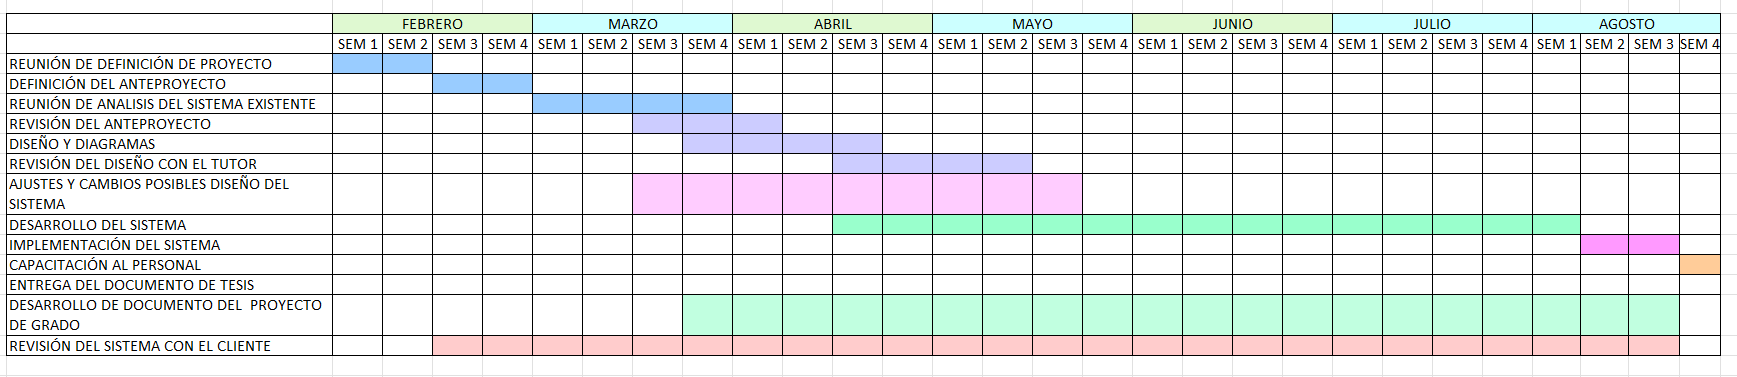
\includegraphics[width=1\linewidth]{img/cronograma.png}
    \caption[Cronograma de Actividades]{Cronograma de Actividades}
    \label{fig:cronograma}
\end{figure}

% Cronograma
\newpage
\section{PRESUPUESTO}
En esta sección se describen los costos proyectados y la inversión en recursos y materiales, con el objetivo de garantizar una gestión responsable de los recursos.

\begin{figure}[htpb]
    \centering
    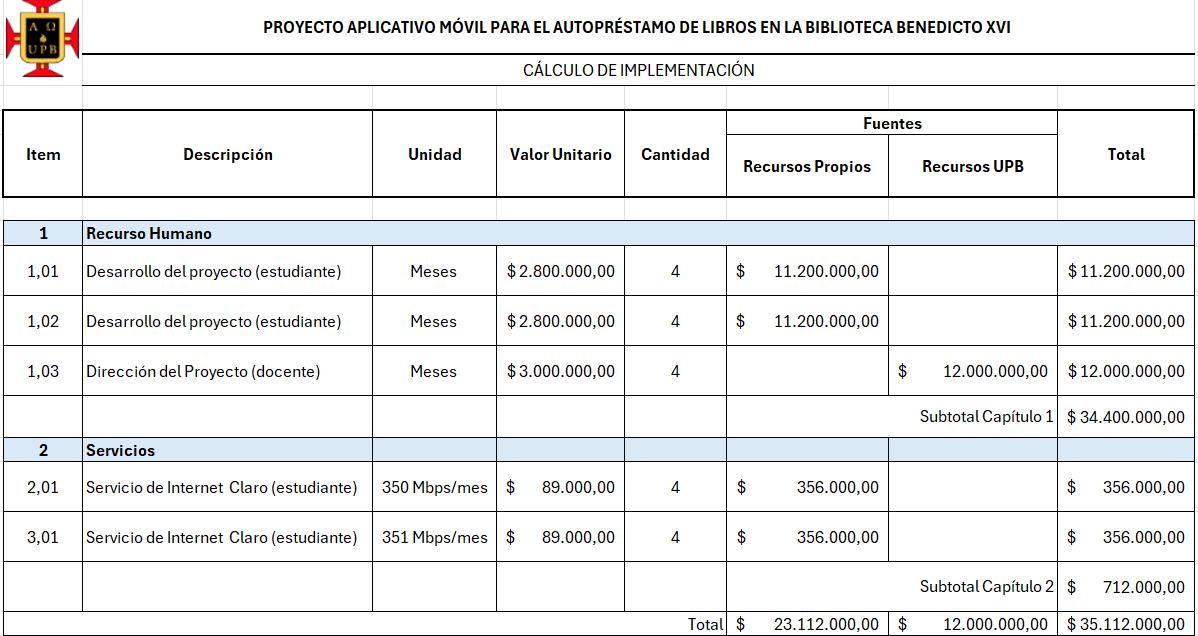
\includegraphics[width=1\linewidth]{img/p.png}
    \caption[Presupuesto]{Presupuesto}
    \label{fig:presupuesto}
\end{figure}


% Resultados
\newpage
\section{RESULTADOS}
\subsection{Primera Fase: Planificación}
\subsubsection{Identificar las necesidades:}
El proceso actual de préstamo de la Biblioteca Benedicto XVI se realiza de forma manual, en donde el usuario de biblioteca (estudiante de pregrado o posgrado, administrativos y docentes) lleva el ejemplar del libro a la ventanilla de circulación y préstamo, para que el funcionario de biblioteca realice el proceso de préstamo por medio del software de Alejandría.  Por parte de Jefatura de Biblioteca (cliente) presentó por medio de un Excel \textit{figura \ref{fig:excelNecesidades}}, las características que la aplicación debería tener. 

\begin{figure}[htpb]
    \centering
    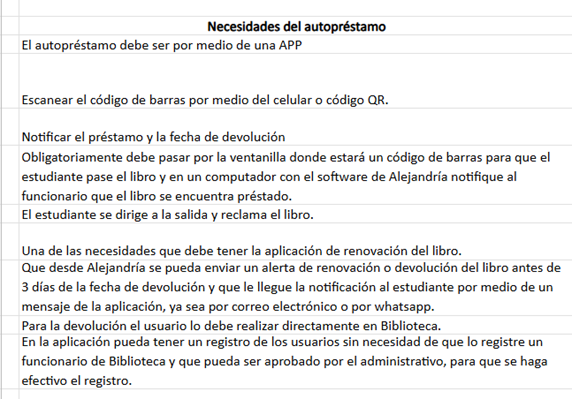
\includegraphics[width=0.7\linewidth]{img/necesidadesAutoprestamo.png}
    \caption[Características Autopréstamo]{Necesidades Autopréstamo Excel}
    \label{fig:excelNecesidades}
\end{figure}

Para identificar cada una de las funcionalidades del aplicativo móvil, se organizaron reuniones periódicas con el cliente, en donde se abordaron cada una de las necesidades expuestas en la \textit{figura \ref{fig:excelNecesidades}}, con el objetivo de resolver las inquietudes respecto a ellas y determinar las características de cada módulo del aplicativo.
\vspace{0.3 cm}

Se determinó que la aplicación móvil únicamente tendría la funcionalidad de prestar libros, y no otros materiales (por ejemplo, portátiles), porque Jefatura prefiere que el préstamo de ese tipo de recursos siga realizándose de manera manual y con un bibliotecario de por medio, principalmente para llevar un control más riguroso.
\vspace{0.3 cm}

Por otra parte, la funcionalidad de registro no se implementará en el aplicativo móvil; se seguirá realizando de forma manual y presencial en la biblioteca, ya que el sistema Alejandría no cuenta con un mecanismo para comprobar la autenticidad de los datos que proporcione el usuario, lo que podría dar lugar a la creación de cuentas falsas.
\vspace{0.3 cm}

 Otra funcionalidad es un sistema automatizado de notificación de renovación de libros. Actualmente, este proceso se realiza de forma manual: la jefa de biblioteca o el administrativo encargado ejecuta una consulta SQL directamente sobre la base de datos para identificar a los usuarios cuyos préstamos están por vencer y, a continuación, les envía un correo. 

\subsubsection{ Planteamiento de las historias de usuario:}
 A partir de las reuniones y el Excel se  definieron las historias de usuario, se pueden visualizar en el anexo \ref{anexos:historias}, en donde se expresaron cada una de las necesidades del cliente.  Su realización fue supervisada por el director del proyecto y posteriormente aprobadas por jefatura de biblioteca.

 \begin{table}[]
    \begin{tabular}{|c|ll|ll|ll|}
        \hline
        \textbf{ÉPICAS} & \multicolumn{2}{c|}{\textbf{Módulo Autopréstamo}}  & \multicolumn{2}{l|}{\textbf{Modulo de Renovación}} & \multicolumn{2}{l|}{\textbf{Módulo de Consultar Libros}}  \\ \hline
        \multirow{5}{*}{\textbf{\begin{tabular}[c]{@{}c@{}}Historias de \\ Usuario\end{tabular}}}
    \end{tabular}
    
 \end{table}


\subsubsection{ Planteamiento de los requerimientos del sistema:}
 Después de establecer las historias de usuario, se realizo el documento de requerimientos de software, el cual se encuentra adjunto en el anexo \ref{anexos:requerimientos}. El documento fue revisado por el director del proyecto de grado y aprobado por jefatura de biblioteca.

\subsection{Segunda Fase Diseño}

\subsubsection{Diseño inicial de UX del sistema:}
 Se presentó al cliente un diseño inicial del sistema, como se puede ver en las figuras \ref{fig:UX1}, \ref{fig:UX2}, \ref{fig:UX3}. Sin embargo, para seguir con los colores institucionales el diseñador de la universidad sugirió unos cambios en la paleta, pero siguiendo la estructura inicial de la aplicación, como se observan en las figuras \ref{fig:UX4}, \ref{fig:UX5}.

 \begin{figure}[H] 
	\centering
	\includegraphics[width=0.6\linewidth]{img/diseñoUXuno.png}
	\vspace{-1mm}
	\caption[Diseño inicial de UX Inicio de Sesión y Menú]{\textit{Se diseña la primera vista inicial del login y menú.}}
	\label{fig:UX1} 
\end{figure}

 \begin{figure}[H] 
	\centering
	\includegraphics[width=0.7\linewidth]{img/diseñoUXdos.png}
	\vspace{-1mm}
	\caption[Diseño inicial de UX Lista de Préstamos]{\textit{Se diseña la primera vista inicial de lista de préstamos.}}
	\label{fig:UX2} 
\end{figure}

 \begin{figure}[H] 
	\centering
	\includegraphics[width=0.5\linewidth]{img/diseñoUXtres.png}
	\vspace{-1mm}
	\caption[Diseño inicial de UX Preguntas Frecuentes]{\textit{Se diseña la primera vista inicial de preguntas frecuentes}}
	\label{fig:UX3} 
\end{figure}

 \begin{figure}[H] 
	\centering
	\includegraphics[width=0.7\linewidth]{img/diseñoUXcuatro.png}
	\vspace{-1mm}
	\caption[Diseño inicial de UX diseñador Login, Menú y Preguntas frecuentes]{\textit{Diseño por parte de la Universidad}}
	\label{fig:UX4} 
\end{figure}

\begin{figure}[H] 
	\centering
	\includegraphics[width=0.7\linewidth]{img/dieñoUXcinco.png}
	\vspace{-1mm}
	\caption[Diseño inicial de UX diseñador Lista de Préstamos]{\textit{Diseño por parte de la Universidad}}
	\label{fig:UX5} 
\end{figure}
% Discusión
\newpage
\section{DISCUSIÓN}
Texto de la discusión... Por ejemplo, según \cite{singh2023mobile}, las aplicaciones móviles han transformado los servicios bibliotecarios.

% Conclusiones
\newpage
\section{CONCLUSIONES}
Texto

% Recomendaciones
\newpage
\section{RECOMENDACIONES}
Texto de las recomendaciones...

\newpage
\renewcommand\refname{REFERENCIAS}
\bibliographystyle{IEEEtran}
\bibliography{bibliography}
\addcontentsline{toc}{section}{REFERENCIAS}

% Anexos
\newpage

%\addcontentsline{toc}{section}{ANEXOS}
%\begin{center}
%\textbf{ANEXOS}
%\end{center}

\appendix
\section{ANEXOS}
\raggedright\textit{\textbf{ANEXO A} HISTORIAS DE USUARIO DEL SISTEMA}
\label{anexos:historias}

A continuación, en las siguientes páginas, se encuentra el documento de las historias de usuario del sistema. 

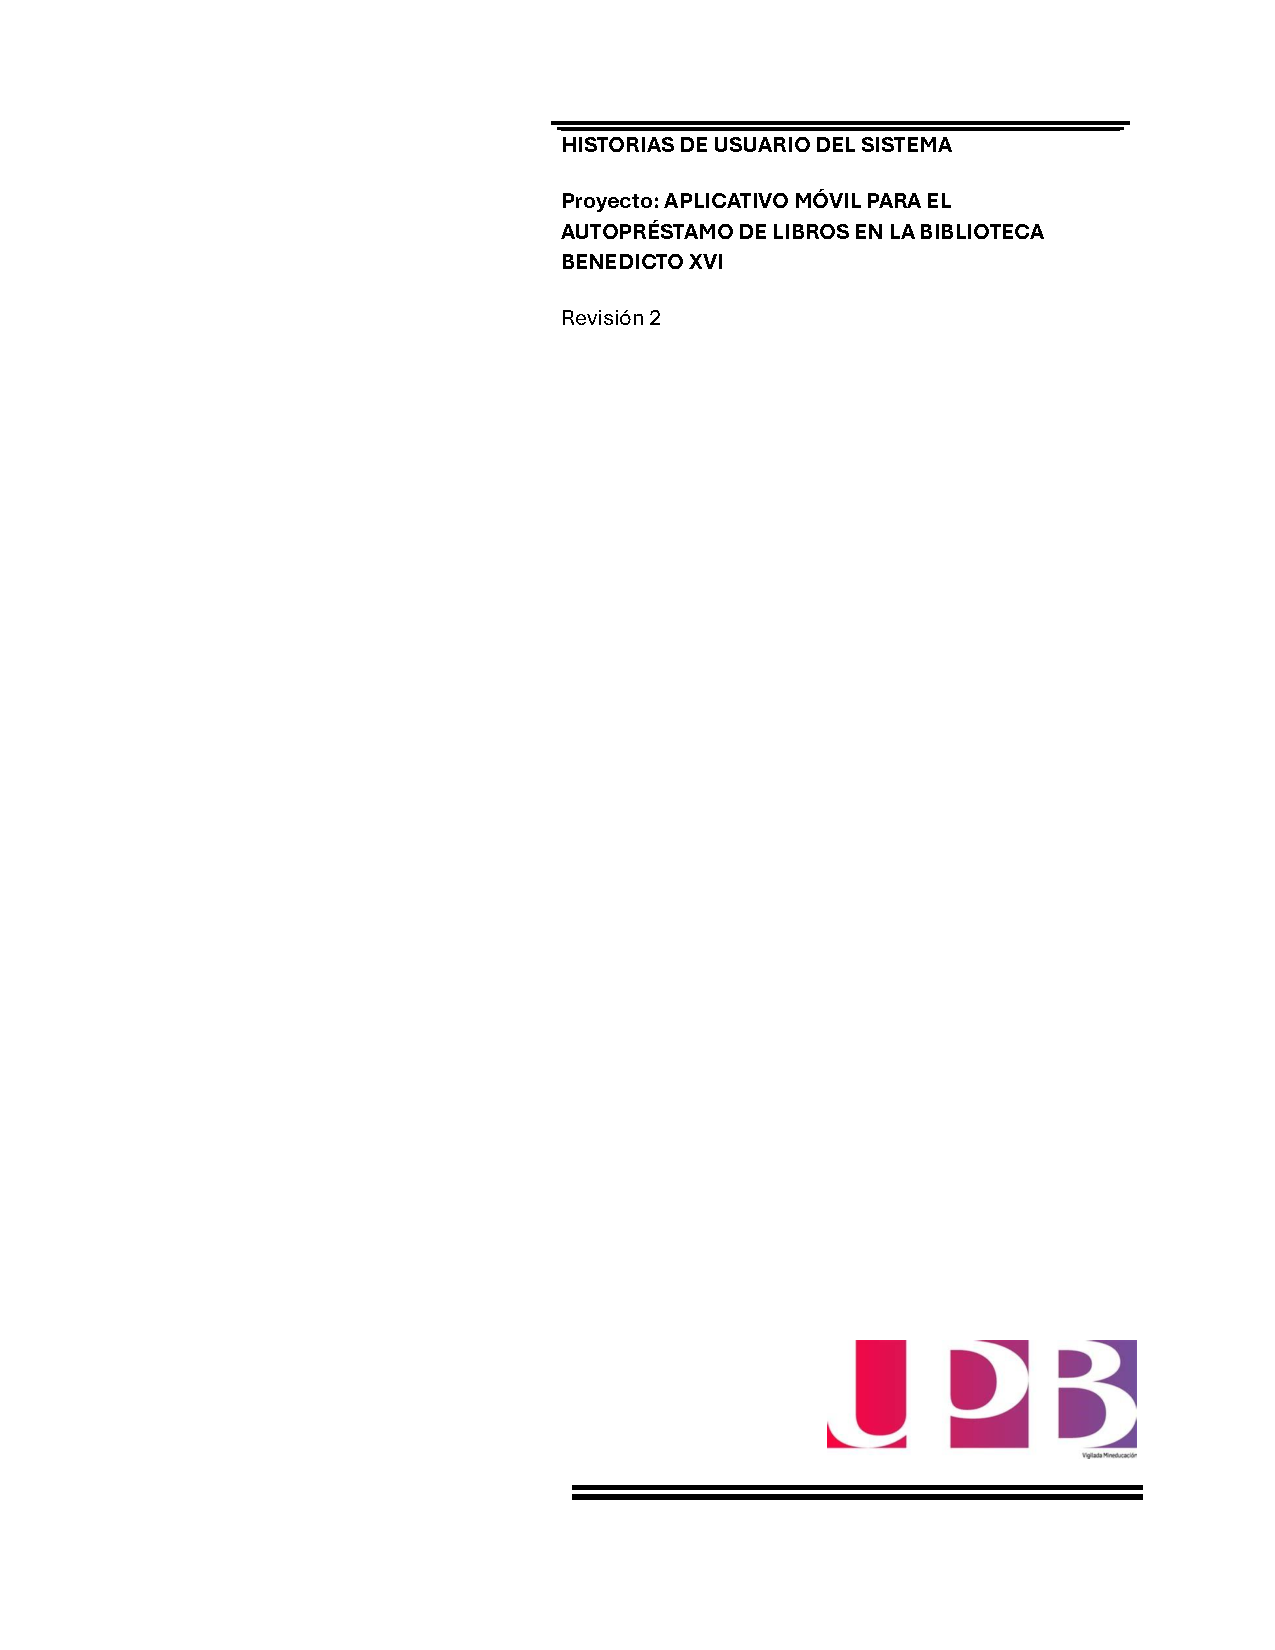
\includepdf[pages=-, fitpaper]{pdfs/historias_usuario.pdf}



\newpage

\section{ANEXOS}
\raggedright\textit{\textbf{ANEXO B} DOCUMENTO DE ESPECIFICACIÓN DE REQUERIMIENTOS FUNCIONALES Y NO FUNCIONALES}
\label{anexos:requerimientos}

A continuación, en las siguientes páginas, se encuentra el documento de especificación de requerimientos funcionales y no funcionales del sistema.

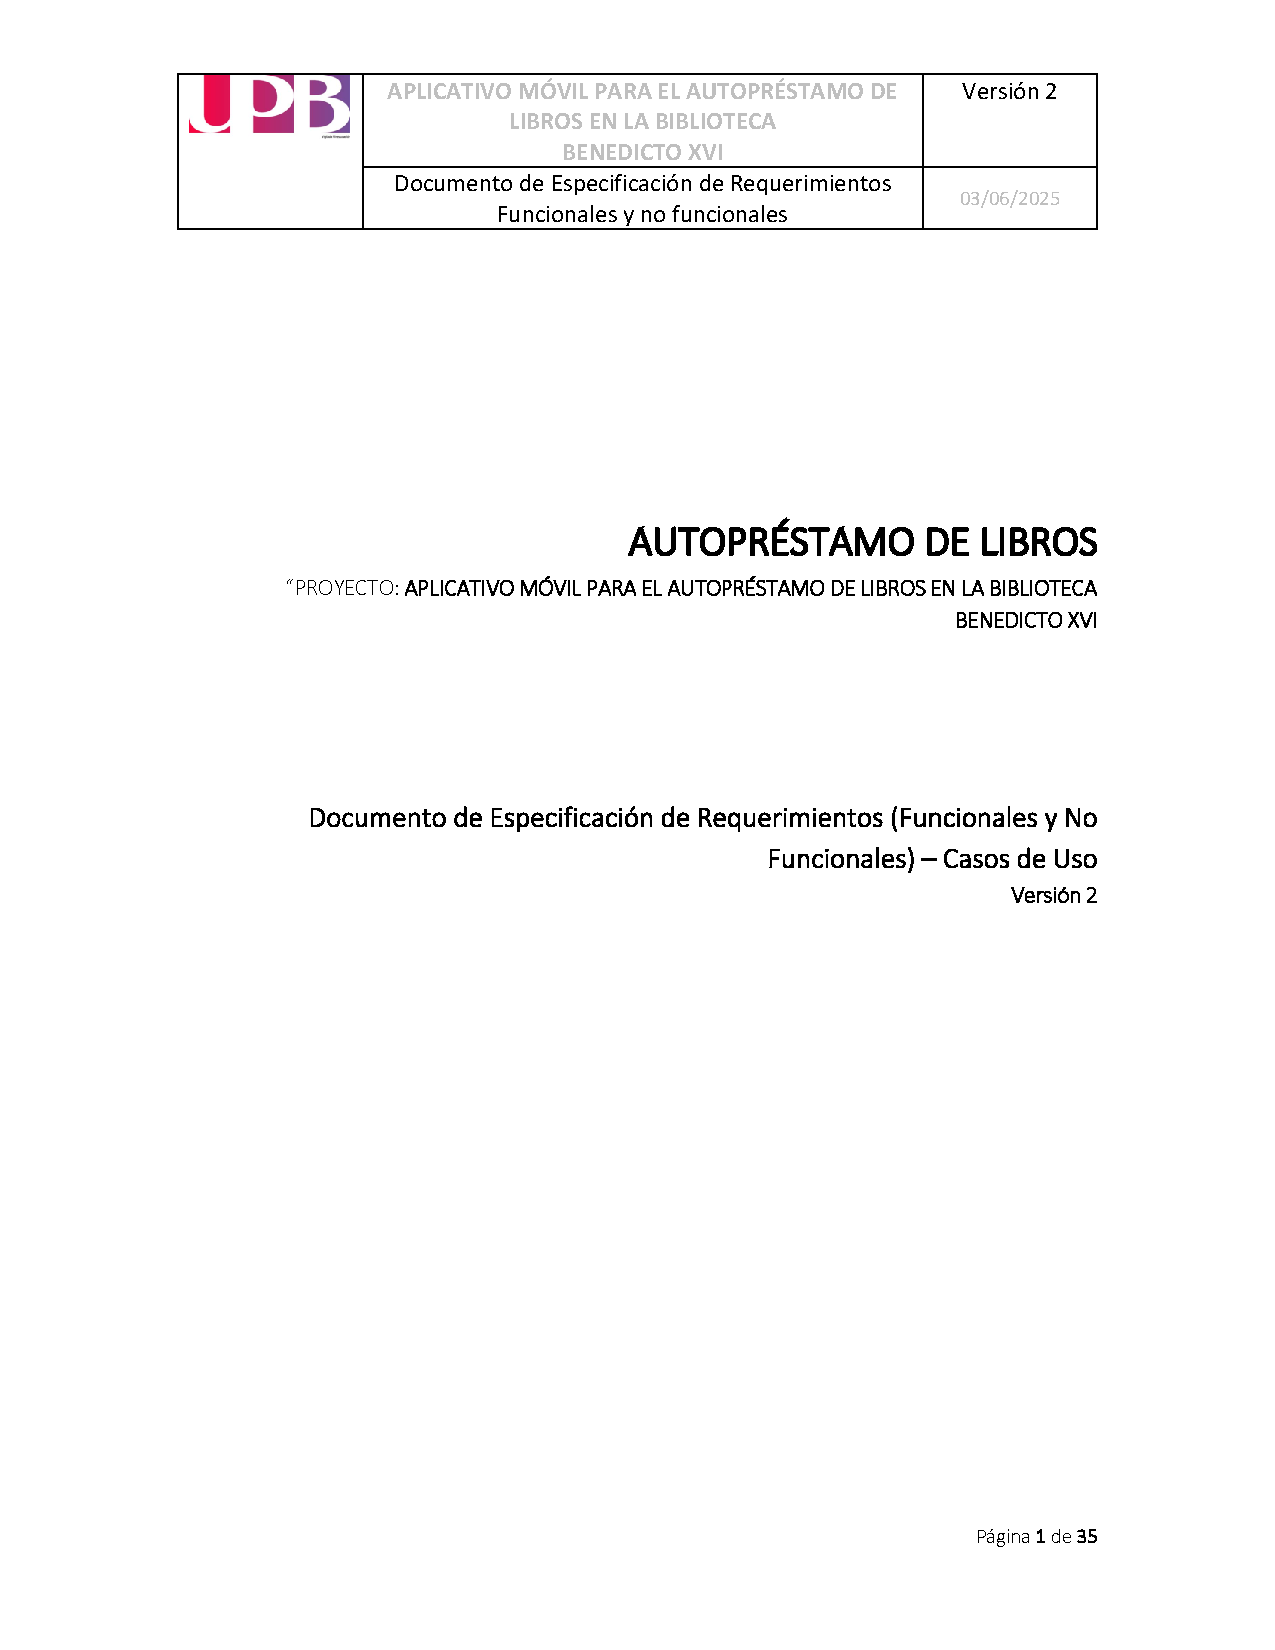
\includepdf[pages=-, fitpaper]{pdfs/Requerimientos2.pdf}

\end{document}
